\section{Theorie}

Um den  Leser  den Einstieg in die Thematik zu erleichtern, wird zuerst einmal
aufgezeigt, um  was  es  sich bei einem Stubfilter genau handelt. Im Anschluss
wird  das  typische  Vorgehen  einer  Filterdimensionierung  beschrieben,  mit
welchem ein Stubfilter realisiert werden kann.

\subsection{Prototypfilter}

Bei jeder Filterdimensionierung wird von einem Prototypfilter ausgegangen, welches üblicherweise in der Form eines normierter Tiefpassfilters vorliegt. Abb.\ref{fig:Prototyp_Filter} zeigt die Topologie eines möglichen Tiefpassfilters (a) mit zugehöriger dualer Topologie (b).

\begin{figure}[h!]
\centering
 	\includegraphics[width=0.5\textwidth]{Prototyp_Filter.png}
 	\caption{Prototypfilter (Tiefpass)}
 	\label{fig:Prototyp_Filter}
\end{figure}

%Quelle : Microwave Filters Impadance Matching Networks and Coupling Structures, P95, Fig4.04-1

Die Werte $g_0$ bis $g_{n+1}$ sind die Elementwerte des Protottypfilters. Diese Elementwerte können aus Tabellen entnommen werden und sind so normiert, dass das beschriebene  Prototypfilter die Grenzfrequenz $\omega_{C} = 1$, sowie die Lastimpedanz (oder Lastadmittanz) von $g_{n+1}=1\Omega$ aufweist. Dadurch kann der Prototyp sehr einfach in ein konkretes LC-Filter mit dem gewünschten Quellenwiderstand und Grenzfrequenz umgerechnet werden. 

Die Umrechnung in ein konkretes LC-Filter mit einer Lastimpedanz $Z_0$ und einer Grenzfrequenz $\omega_{C} = 1$ wird auch Entnormierung genannt und kann mit folgenden Formeln bewerkstelligt werden: 

\begin{equation}\label{eq:R}	
R_i = R'_i \cdot Z_0
\end{equation}

\begin{equation}\label{eq:L}	
L_i = \frac{L'_i \cdot Z_0}{\omega_{C}}
\end{equation}

\begin{equation}\label{eq:C}	
C_i = \frac{C'_i}{Z_0 \cdot \omega_{C}}
\end{equation}

Dabei beschreiben  $R'_i$, $C'_i$ und $L'_i$ die normierten Elementwerte  $g_0$ bis $g_{n+1}$ und $R_i$, $C_i$, und $L_i$ die konkreten Werte nach der Entnormierung.


Bei jeder Filterdimensionierung wird von einem Prototypfilter ausgegangen, welches üblicherweise in der Form eines normierter Tiefpassfilters vorliegt. Abb.\ref{fig:Prototyp_Filter} zeigt die Topologie eines normierten Tiefpassfilters (a) mit zugehöriger dualer Topologie (b).

\begin{figure}[h!]
\centering
 	\includegraphics[width=0.5\textwidth]{Prototyp_Filter.png}
 	\caption{Prototypfilter (Tiefpass)}
 	\label{fig:Prototyp_Filter}
\end{figure}

Die Werte $g_0$ bis $g_{n+1}$ sind die Elementwerte des Protottypfilters. Diese Elementwerte können aus Tabellen entnommen werden und sind so normiert, dass das beschriebene  Prototypfilter die Grenzfrequenz $\omega_{C} = 1$, sowie den Quellenwiderstand $g_{n0}=1$ aufweist. Dadurch kann der Prototyp sehr einfach in ein LC-Filter mit den gewünschte Quellenwiderstand und Grenzfrequenz umgerechnet werden. 

Die folgenden Formeln zeigen, wie eine solche Entnormierung durchgeführt wird:


\begin{equation}\label{eq:Z(s)}	
	\underline{Y'}(s) = \underline{Z}(s)	
\end{equation}



\subsection{Stubfilter}

Im Kapitel \ref{Protototypfilter} wurde gezeigt, wie durch die Entnormierung eines Prototypfilter ein konkretes LC-Filter dimensioniert werden kann. Solche LC-Filter  können in einem weiten Frequenzbereich  eingesetzt  werden.  Jedoch
wird  bei realen konzentrierten Elementen (R,L,C) zu höheren Frequenzen hin der Einfluss der parasitären Eigenschaften immer deutlicher, so dass hohe Anforderungen an die Bauteilgüte  gestellt  werden  müssen. Im GHZ-Bereich wird es daher  zunehmend attraktiv,  statt  konzentrierten  Kapazitäten  und  Induktivitäten  verteilte
Strukturen  in  Form  von  Leitungen  zu  verwenden.  Man  spricht   dann  von sogenannten Leitungsfiltern.
%Quelle direktes Zitat: 
%https://books.google.ch/books?id=MTVQAgAAQBAJ&pg=PA203&lpg=PA203&dq=leitungsfilter+hochfrequenztechnik&source=bl&ots=Ljf0GRJkZt&sig=n-0G9H5VZ9iuPc2qepAATnjA47M&hl=de&sa=X&ved=0ahUKEwj38u-T79DUAhUSL1AKHUsyDNMQ6AEINTAB#v=onepage&q=leitungsfilter%20hochfrequenztechnik&f=false%

Es gibt verschiedene Arten um  Leitungsfilter zu realisieren. Eine Möglichkeit der  Realisierung  ist das Stubfilter.  Dieses  Filter  verwendet  gleichlange kurzgeschlossenen Leitungen (TLSC) und  leerlaufende  Leitungen(TLOC), welche an einem Ende verbunden und am anderen Ende entweder kurzgeschlossen
oder offen gelassen werden. Diese sogenannten Stubs oder Stichleitungen werden mit gleichlangen Verbindunsleitungen (TLIN) verbunden. 

In Abb. \ref{fig:Stubfilter} ist ein solches Stubfilter zu sehen, welches aus 8 kurgeschlossenen Stubs (TLSC) besteht.

\begin{figure}[h!]
\centering
 	\includegraphics[width=0.5\textwidth]{Stripline_Stub_Filter.png}
 	\caption{Stubfilter}
 	\label{fig:Stubfilter}
\end{figure}

%Quelle: Wikipedia https://en.wikipedia.org/wiki/File:Stripline_stub_filter.svg

Stubs verhalten sich bei  hohen  Frequenzen  wie  reaktive Elemente(L,C) und ermöglichen so die Realisierung  eines  Mikrowellenfilters. Für Stubfilter existiert eine geschlossene Thoerie zur Filtersynthese. Dadurch muss ein herrkömmliches Prototypfilter nur entnormiert und transformiert werden, um das gewünschte Stubfilter mit den gewünschten Eigenschaften zu erhalten.


\subsection{Richards Frequenztransformation}

Der  Frequenzbereich von konzentrierten LC-Filtern ist beschr\"ankt durch  die
Nichtidealit\"at der Komponenten.  W\"ahrend  die  Reaktanz und die G\"ute von
konzentrierten Induktivit\"aten und Kapazit\"aten  im  Bereich  \"uber  einige
\SI{100}{\mega\hertz} keinen hohen Filteranspr\"uchen mehr gen\"ugen k\"onnen,
w\"aren die entsprechenden Reaktanzen noch  sehr gut mit verteilten Elementen,
wie   leerlaufenden   und   kurzgeschlossenen  Leitungen  sowie  verschiedenen
gekoppelten   Leitungen  realisierbar.   Es   ist   beispielsweise   aus   der
Leitungstheorie  bekannt,  dass  leerlaufende  Leitungen   mit  einer  L\"ange
$l\le\frac{\lambda}{4}$   kapazitiv   und   kurzgeschlossene   Leitungen   mit
$l\le\frac{\lambda}{4}$  induktiv  sind.  Wir  k\"onnten damit die  induktiven
Reaktanzen und  die  kapazitiven  Suszeptanzen  mit  solchen Leitungselementen
ersetzen.

\begin{figure}
    \centering
    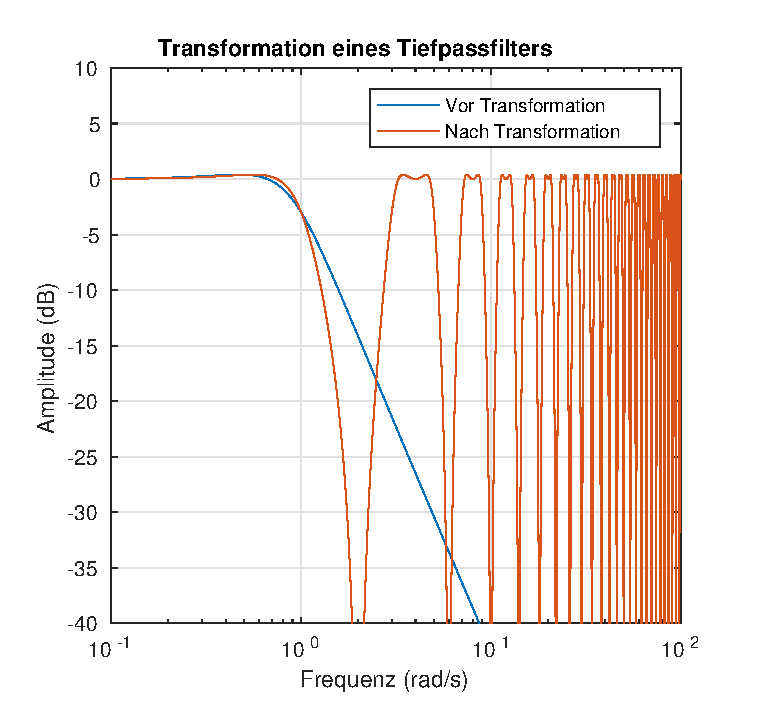
\includegraphics[width=\imagewidth]{images/richards-lowpass-example}
    \caption{Richards Frequenztransformation eines Chebychev-Tiefpassfilters (3. Ordnung)}
    \label{fig:richards-example}
\end{figure}

Dies wird mithilfe der sogenannten \textit{Richards Frequenztransformation} erreicht. 

\subsection{Kuroda Transformation}

Die   Umwandlung   von   LC-Filter   in   Leitungsfilter    ist    dank    der
Richards-Transformation recht einfach, jedoch  wird  man  bei der Realisierung
als Mikrostreifenfilter auf Probleme stossen.

\begin{figure}[h!]
    \centering
    \includegraphics[width=\imagewidth]{images/mikrostreifen}
    \caption{Auszug aus dem Buch Mikrowellentechnik\cite[p.~27]{ref:baechold}: Realisierung von Stichleitungen in Mikrostreifentechnik: a: leerlaufende, geerdete Leitung und b: kurzgeschlossene, erdfreie Leitung}
    \label{fig:mikrostreifen}
\end{figure}

Gem\"ass Abbildung \ref{fig:mikrostreifen}a  kann  die  leerlaufende, geerdete
Stichleitung  als  Einzelleitung  recht  gut  in  Mikrostreifentechnik  gebaut
werden.  Nach Abbildung \ref{fig:LC-zu-Leitungsfilter} sollten die Leitungen 1
und 3 am Fusspunkt  der  kurzgeschlossenen  Stichleitung  2,  also mit kleinem
gegenseitigem  Abstand, angeschlossen werden. Da  eine  gegenseitige  Kopplung
zwischen  1  und  3  unerw\"unscht  ist,  f\"uhrt diese enge Nachbarschaft  zu
Problemen.  Die  kurzgeschlossene  Stichleitung  2 l\"asst sich, wie Abbildung
\ref{fig:mikrostreifen}b zeigt, nur schlecht realisieren.  Die  Induktivit\"at
sollte  in  Form  einer  erdfreien, kurzgeschlossenen Stichleitung erscheinen.
Eine  elektrisch  und  geometrisch  wenig  befriedigende  Anordnung ist in der
Abbildung \ref{fig:mikrostreifen}b  gezeigt,  wo  mit  einer  \"Offnung in der
Grundplatte eine gewisse Erdfreiheit erzielt wird. Dieses Beispiel zeigt, dass
die   vorliegende   Tiefpassstruktur   nicht   f\"ur  eine   Realisierung   in
Mikrostreifentechnik   geeignet  ist.  Es  w\"are  von   Vorteil,   wenn   nur
kurzgeschlossene  oder  leerlaufende  Stichleitungen  gegen   die  Grundplatte
auftreten  w\"urden.  Weiter   w\"are   eine   gewisse  Distanz  zwischen  den
Leitungselementen  vorteilhaft,  um  unerw\"unschte  Kopplungen zu  vermeiden.
Genau  diese  Anspr\"uche  werden  weitgehend  mit  der  Kuroda-Transformation
befriedigt, wie nachfolgend gezeigt wird.

Neben den kurzgeschlossenen und leerlaufenden  Stichleitungen f\"uhren wir als
zus\"atzliches  Leitungselement das Einheitselement (unit element)  U.E.  ein,
welches  ein  St\"uck  \"Ubertragungsleitung mit einer Wellenimpedanz $Z_{ue}$
und der gleichen L\"ange $I$ wie die Stichleitungen darstellt.

\begin{figure}[h!]
    \centering
    \includegraphics[width=\imagewidth]{images/kuroda-identities}
    \caption{Kuroda-Identit\"aten}
    \label{fig:kuroda-identities}
\end{figure}

In     der     Abbildung    \ref{fig:kuroda-identities}    sind    die     von
Kuroda\cite{ref:kuroda} formulierten Identit\"aten.  Damit  kann  zum Beispiel
mit   der   vierten  Identit\"at   eine   schlecht   realisierbare   erdfreie,
kurzgeschlossene  Stichleitung   in   eine   einfach  realisierbare  geerdete,
leerlaufende    Stichleitung    umgeformt    werden.    Wir   benützen   diese
Kuroda-Transformation,  um  den in  der  Richards-Transformation  entstandenen
Tiefpassfilter  in  eine  realisierbare  Topologie umzuformen.  Die  Abbildung
\ref{fig:kuroda-schieben}   zeigt   den   Vorgang   anhand   eines   einfachen
Tiefpass-Filters.

\begin{figure}[h!]
    \centering
    \includegraphics[width=.8\linewidth]{images/kuroda-schieben}
    \caption{Beispiel einer Umwandlung von schlecht realisierbaren Leitungsst\"ucken mithilfe der Kuroda-Transformation}
    \label{fig:kuroda-schieben}
\end{figure}




% TODO Move this somewhere else
\subsection{Ablauf Filterdimensionierung}

Der grundsätzliche Vorgehen bei der Filterdimensionierung ist bei fast allen Filtertypen gleich. Deshalb wird zuerst der allgemeinen Ablauf(Abb.\ref{fig:Ablauf_Filterdimensionierung_Allgemein}) der Filterdimensionierung beschrieben 

Der Entwurfsprozess jedes Filters beginnt mit der Filterspezifikation, welche mathematisch mit einer Funktion im Prototypbereich T(s) beschrieben wird. Aus dieser Funktion kann mit Hilfe einer Filtersynthese (rot) eine realisierbare Filterstruktur gefunden werden. Dabei ist zu beachten, dass  physikalische Randbedingungen einbezogen werden müssen, die nicht beliebig steile und beliebig verlustfreie Filtercharakteristiken erlauben.

Die Filtersynthesen unterschiedlicher Realisierungen haben gemeinsam, dass sie alle auf der klassischen LC-Filtersynthese basieren. Nach der LC-Filtersynthese liegt ein LC-Prototypfilter vor. Dieses LC-Prototypfilter wird bei der anschliessenden Filter-Realisierung mithilfe von unterschiedlichen Transformationen in den gewünschten Filter-Typ überführt(falls nötig). Für Elektroingenieure bekannte Transformationen sind z.B die billineare und die impulsinvariante Transformation, welche zur Überführung von einem LC-Filter in ein digitales Filter verwendet werden. Nach der Transformation ist die Filtersynthese abgeschlossen. Zuletzt wird das Filter aufgebaut wenn bei der Analyse alle Spezifikationen eingehalten wurden.

\begin{figure}[h!]
\centering
 	\includegraphics[width=0.5\textwidth]{Ablauf_Filterdimensionierung_Allgemein.png}
 	\caption{Ablauf Filterdimensionierung}
 	\label{fig:Ablauf_Filterdimensionierung_Allgemein}
\end{figure}

%Liegen keine speziellen Anforderungen an das Filter vor, so können Standardfilter(Butterworth, Chebyshev, Bessel und Cauer)verwendet werden. Die Reaktanzwerte, welche für die Beschreibung der Übertragungsfunktion des LC-Prototypfilters notwendig sind, sind aus Tabellen zu entnehmen. Werden Spezielle Anforderungen an das Filter gestellt, so eignen sich die Standardfilter nicht und es muss eine LC-Filtersynthese durchgeführt werden.

\paragraph{Realisierung Stubfilter}

Um schlussendlich vom LC-Prototypfilter zu einem realisierebaren Stubfilter zu gelangen sind zwei Transformationen notwendig: Die Richard's Transformation und die Kuroda Transformation.

Mit der Richard's Transformation können die konzentrierten Elemente (L,C) des Prototypfilter mit verteilte Elementen (Stubs) ersetzt werden. Nach dieser Transformation spricht man von einem Stubfilter. Das Problem ist aber, dass sich dieses Filter nicht realisieren lässt, weil sich alle Stubs am gleichen Ort befinden. 

Deshalb wird im Anschluss die Kuroda Transformation verwendet,  um eine physikalische Distanz zwischen
den  Stubs  zu  schaffen, damit das Filter auch in Realit\"at umgesetzt  werden  kann.

